\documentclass[
    ../../Software_Engineering_Summary.tex,
]
{subfiles}

\externaldocument[ext:]{../../Software_Engineering_Summary.tex}
% Set Graphics Path, so pictures load correctly
\graphicspath{{../../}}

\begin{document}
\section{Verification}
\subsection{Introduction}
\subsubsection{Validation vs. Verification}

\begin{defbox}
    [Validation]
    \defc{Validation} ensures that the software meets the costumers expectation.
    \begin{center}
        \begin{smalldefbox*}
            Are we building the \defc{right} system?
        \end{smalldefbox*}
    \end{center}

    \begin{itemize}
        \item Is the feature set as intended and complete?
        \item Does it fit into the organizations workflow?
    \end{itemize}

    Validation is reliant on correctly performed requirements analysis and thus cannot be done without involving the user / customer.
\end{defbox}

\begin{defbox}
    [Verification]
    \defc{Verification} ensures that the software is correct in respect to the system specification.
    \begin{center}
        \begin{smalldefbox*}
            Is the system built \defc{right}?
        \end{smalldefbox*}
    \end{center}

    \begin{itemize}
        \item Do the features work as specified?
        \item How does the system react to faults?
    \end{itemize}

    Verification is performed in solution space by the developer and thus doesn't necessarily involve the user.
\end{defbox}

\subsubsection{Verification Techniques}
\begin{defbox}
    [Static]
    Static techniques do not require code execution.
    \begin{itemize}
        \item \defc{Code Review:} Can be done at any stage of development
        \item \defc{Static Checking:} Automated analysis of source code (Type checks, bug finders, etc.)
        \item \defc{Formal Verification:} Ensures that a program satifies a formal specification
    \end{itemize}
\end{defbox}

\begin{defbox}
    [Dynamic]
    Dynamic techniques require code execution.
    \begin{itemize}
        \item \defc{Testing:} Assert correct behavior for specific inputs
        \item \defc{Runtime Monitoring:} Instrument program with safety assertions, whose violations are detected at runtime 
    \end{itemize}
\end{defbox}

\subsection{Code Review}
\begin{defbox*}
    A \defc{Code Review} is an inspection process in which a team reviews project code, with the goal of identifying errors, bugs, deviations from conventions, etc.
\end{defbox*}

\subsubsection{Building Blocks}
In a code review all team members take on specific roles:
\begin{itemize}
    \item \defc{Author / Owner:} Writing the code
    \item \defc{Inspector / Reader:} Inspecting the code
    \item \defc{Scribe:} Writing down comments, questions, requirements, etc.
    \item \defc{Chair / Moderator:} Leads project and manages discussion and requirements
\end{itemize}

\begin{figure}
    [H]
    \centering
    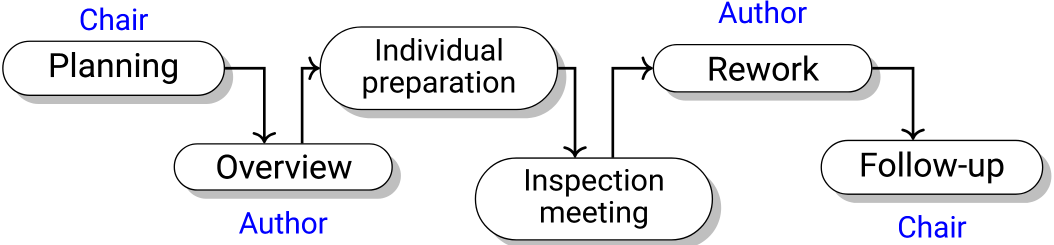
\includegraphics[width = 0.7\textwidth]{Pics/10/CodeReviewBuildingBlocks.png}
\end{figure}

\subsubsection{Check Lists}
Code Reviews are often driven by a \defc{Check List}, which is used to specify specific fault classes that should be checked. These are often individual to the project environment based on language, coding standards, etc. 

\begin{defbox}
    [Check List Example]
    \begin{tabular}{r l}
        \defc{Data Fault} & Are all variables initialized? \\
        \defc{I/O Fault}  & Are all input variables used? \\
        \defc{\dots}      & \dots \\
    \end{tabular}
\end{defbox}

\begin{defbox}
    [Advantages]
    \begin{itemize}
        \item Empirical evidence that they work and save cost
        \item Distribute knowledge of the codebase to all team members
        \item Find defects before they might cause problems in tests
        \item Improves code quality
        \item Code does not need to be executed
    \end{itemize}
\end{defbox}

\begin{defbox}
    [Disadvantages]
    \begin{itemize}
        \item Team members might feel criticized
        \item Time pressure might become worse because of the review
        \item Only works when properly conducted
    \end{itemize}
\end{defbox}

\subsection{Software Testing}
Testing can never show all faults, but it can reduce them. (\href{https://en.wikipedia.org/wiki/Falsifiability}{Falsifiability})

\subsubsection{Constituents}
\begin{defbox*}
    \begin{itemize}
        \item \defc{System or Implementation under test (SUT, IUT)}
        \item \defc{Test Inputs}
        \item \defc{Test Harness:} Runtime environment, preparation and execution, clean up
        \item \defc{Test Verdict:} Given by \defc{Test Oracle}
    \end{itemize}
\end{defbox*}

\subsubsection{Test Levels}
\begin{figure}
    [H]
    \centering
    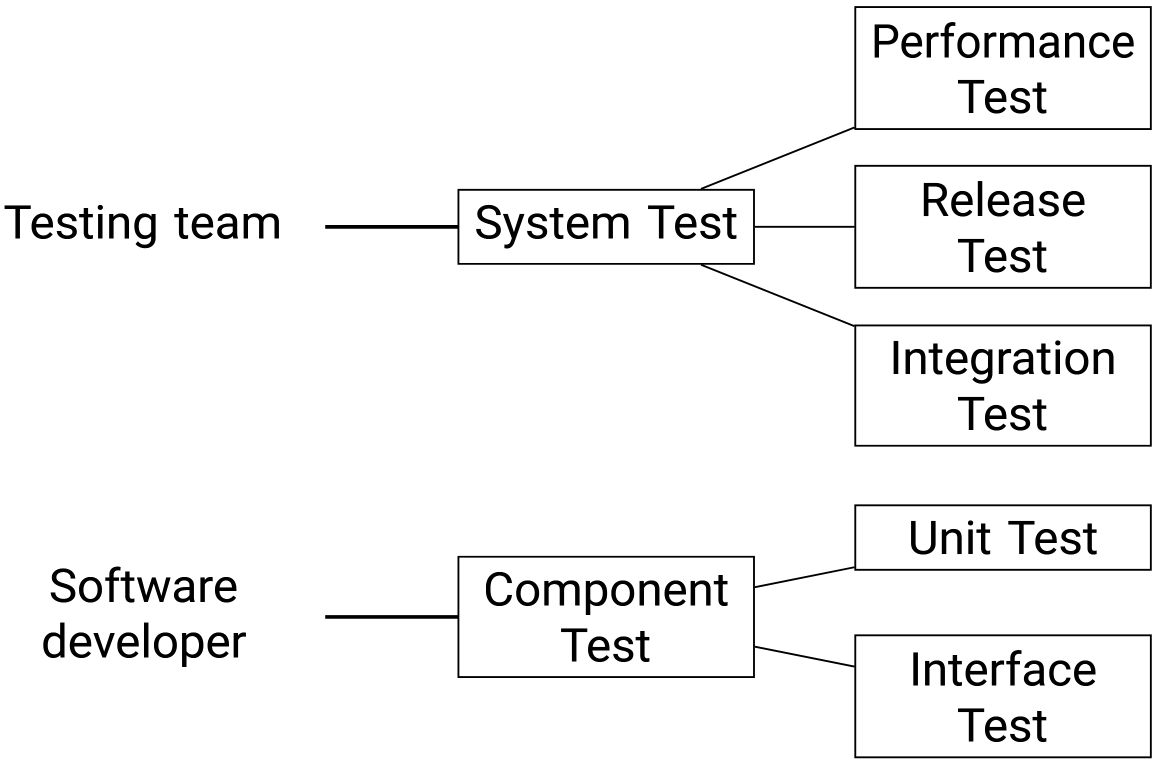
\includegraphics[width = 0.55\textwidth]{Pics/10/TestLevels.png}
\end{figure}

\subsubsection{Test Plan}
A test plan contains detailed descriptions of the testing process. It is a document intended to be read by humans.

\begin{itemize}
    \item \defc{Work Plan:} Phases, schedules, etc.
    \item \defc{Testing Procedures}
    \item Explanation of the \defc{test design}
    \item \textbf{Test documentation just as important as code documentation}
\end{itemize}

\subsubsection{Test Design}
\begin{defbox*}
    \begin{enumerate}
        \item Identify and analyze responsibilities of the IUT
        \begin{itemize}
            \item \defc{Pre- and Postconditions} in use cases
            \item \defc{Minimal and Success Guarantees} in use cases
            \item Analyze distribution of responsibilities
        \end{itemize}
        \item Add test cases based on
        \begin{itemize}
            \item Use Case-, Design- and Code Analysis
            \item Suspicions, minimal success guarantees
            \item General Heuristics (Domain / Expression boundaries)
        \end{itemize}
        \item Determine for each test case how verdict is reached: Provide expected results, programmed or human test oracle
    \end{enumerate}
\end{defbox*}

\subsubsection{Test Automation}
Testing is very expensive; Typically about 15 - 20\% of development costs are allocated towards testing.

These can be reduced automating tests:
\begin{enumerate}
    \item \defc{Running the tests:} Nightly, after each change, etc.
    \item \defc{Generating test cases:} 
    \begin{enumerate}
        \item Code-driven
        \item Model-driven
        \item Data-driven
    \end{enumerate}
    \item \defc{Generating test verdict:}
    \begin{enumerate}
        \item Test oracle as a small program, added to the test harness
        \item Oracle generated automatically from formal specification
    \end{enumerate}
\end{enumerate}

\begin{defbox}
    [Tasks of a Test Automation System]
    \begin{enumerate}
        \item Set up test environment
        \begin{itemize}
            \item Start servers, establish connection, register services
        \end{itemize}
        \item Start IUT
        \item Bring IUT to required pretest state
        \begin{itemize}
            \item Load required data, create required objects
        \end{itemize}
        \item Set tests inputs
        \item Evaluate output and test verdict
        \item Clean up environment
        \begin{itemize}
            \item Delete files, stop services, reset data
        \end{itemize}
    \end{enumerate}

    Not everything is possible to automate, some manual tasks remain (Test inputs, test oracle)
\end{defbox}

\subsubsection{Test Goal}
\begin{defbox*}
    Establish \textbf{sufficient} trust, that system is operational by exercising the interfaces between its parts.
\end{defbox*}

\subsubsection{Test Input}
\begin{defbox}
    [Test (Data) Point]
    A \defc{Test Point} is a specific value for 
    \begin{itemize}
        \item a test case input
        \item a state variable
    \end{itemize}
    The test point is selected from a domain. A \defc{domain} is the set of values that input or state variables can assume.
\end{defbox}

\begin{defbox}
    [Heuristics for Test Point Selection]
    \begin{itemize}
        \item \defc{Equivalence Classes:} Singular test point for expected equivalent outcome
        \item \defc{Boundary Values:} Min/Max of ordered domain, pivot for comparison
        \item \defc{Special values:} Null, other values with specific semantics
    \end{itemize}    
\end{defbox}

\subsubsection{Other Definitions}
\begin{defbox}
    [Test Case]
    A \defc{Test Case} consists of
    \begin{itemize}
        \item Pretest State of IUT
        \item Test Point / Conditions: test input
        \item Expected result
    \end{itemize}
    A collection of test cases is called a \defc{Test Suite}.
\end{defbox}

\begin{defbox}
    [Test Run]
    A \defc{Test Run} is the execution of a test suite on a single IUT.
    A test whose results are equal to the expected results gets the \defc{verdict} \defc{Pass}, otherwise a \defc{Fail}.
\end{defbox}

\begin{defbox}
    [Test Driver \& Test Harness]
    A \defc{Test Driver} is a class or program that applies test cases to an IUT.\\
    A \defc{Test Harness} is a system of test drivers and other components that support test execution.
\end{defbox}

\begin{defbox}
    [Fault \& Failure]
    A \defc{Fault} is missing or incorrect code.\\
    A \defc{Failure} is teh manifested inability of a system to perform a required function within specified limits (Time, memory, etc.)
\end{defbox}

\subsubsection{JUnit Test Framework}
\begin{codebox}
    [Example of JUnit Test]
    \begin{lstlisting}[language=Java]
public class AccountTest {
    Account account;
    @BeforeEach // Runs before each test (Pretest State)
    public void setUp() {
        account = new Account(100);
    }
    @AfterEach // Runs after each test (Cleanup, Posttest State)
    public void tearDown() {
        account = null;
    }
    @Test 
    public void successfulWithdrawTest() {
        assertTrue(account.withdraw(50)); // Delivers a passing verdict if value is true
    }
    @Test
    public void failedWithdrawTest() {
        assertFalse(account.withdraw(150)); // Delivers a passing verdict if value is false
    }
}\end{lstlisting}
\end{codebox}

\newpage
\subsection{Test Coverage}
\subsubsection{When to Stop Testing?}
\begin{defbox}
    [Structural Criteria (Code Structure)]
    Based on the \defc{Control Flow Graph (CFG)} of a program.
    \vspace{10pt}

    \begin{tabularx}{\textwidth}{r X}
        \defc{Statement Coverage (SC)} & Each \defc{statement executed} at least once \\
        \defc{Basic Block Coverage (BBC)} & Each \defc{basic block} executed at least once (implies \defc{SC})\\
        \defc{Branch Coverage (BC)} & Each \defc{outgoing edge} from a node in the CFG is executed at least once (implies \defc{BBC})\\
        \defc{Path Coverage (PC)} & Each \defc{path} through the CFG is executed at least once (implies \defc{BC}), unachievable in practice, \# of paths grows exponentially\\
    \end{tabularx}
\end{defbox}

\begin{codebox}
    [Example of Structural Coverage]
    \begin{minipage}
        [c]{0.28\textwidth}
        \begin{algorithm}[H]
            i = 1\;
            min = a[0]\;
            \While{$i < n$.length}{
                \If{$a[i] <$ min}{
                    min = a[i]\;
                }
                i++\;
            }
            \KwRet min\;
        \end{algorithm}
    \end{minipage}
    \begin{minipage}
        [c]{0.3\textwidth}
        \centering
        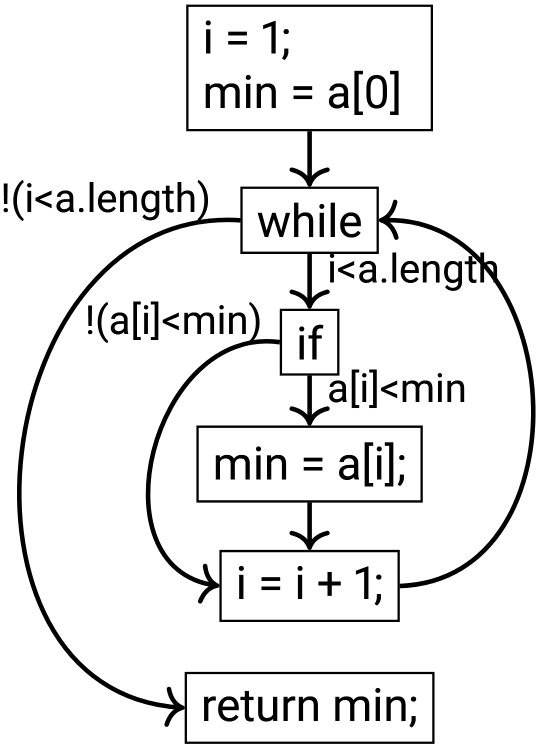
\includegraphics[width=0.8\textwidth]{Pics/10/CFGStructural.png}
    \end{minipage}
    \hfill
    \begin{minipage}
        [c]{0.4\textwidth}
        \begin{defbox}
            [Definitions]
            \begin{tabularx}
                {\textwidth}{p{0.35\textwidth} X}
                \defc{Execution Path} & A complete path through the CFG\\
                \defc{Feasible} & A path that can actually be taken\\
            \end{tabularx}
        \end{defbox}
    \end{minipage}
\end{codebox}

\begin{defbox}
    [Logic-Based Criteria (Logical Case Distinctions)]
    \begin{tabularx}{\textwidth}{p{0.4\textwidth} X}
        \defc{Condition Coverage (CC)} & Each \defc{condition} evaluated as true and as false in at least one test run \\
        \defc{Decision Coverage (DC)} & Each \defc{decision} (guard) evaluated as true and as false in at least one test run \\
        \defc{Modified Condition Decision Coverage (MCDC)} & Combines \defc{CC} and \defc{DC} \& independence test\\
        \defc{Multiple-Condition Coverage (MCC)} & All true-false combinations of conditions are tested in at least one test run\\
    \end{tabularx}
\end{defbox}

\begin{defbox}
    [Condition vs. Decision]
    \begin{tabularx}
        {\textwidth}{p{0.2\textwidth} X}
        \defc{Condition} & A condition is a Boolean Expression \& cannot be divided into sub-expressions\\
        \defc{Decision} & A decision is a Boolean Expression constituting the guard of a conditional or loop statement\\
    \end{tabularx}

    \begin{center}
        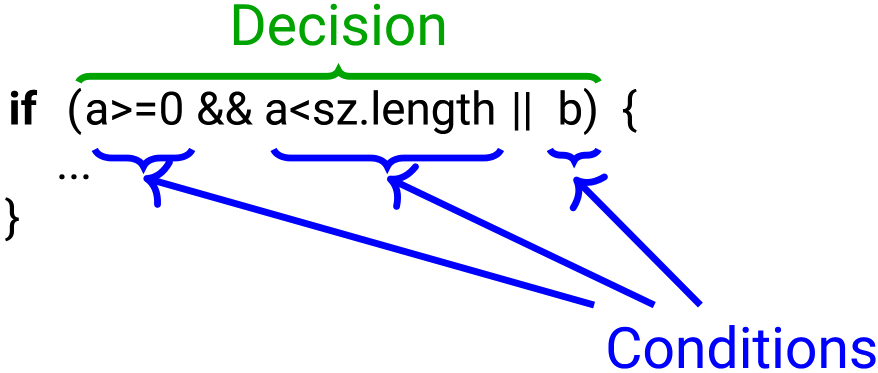
\includegraphics[width=0.4\textwidth]{Pics/10/DecisionCondition.png}
    \end{center}
\end{defbox}

\begin{defbox}
    [Modified Condition Decision Coverage (MCDC)]
    For one occurrence of condition c \textbf{inside} decision d, MCDC is satisfied if:
    \begin{enumerate}
        \item Evaluates d at least twice
        \begin{itemize}
            \item once where c is true
            \item once where c is false
        \end{itemize}
        \item d evaluates differently in both cases
        \item all other conditions in d evaluate identically in both cases \textbf{or} are not evaluated at all in at least one case.
    \end{enumerate} 
\end{defbox}
\end{document}